\documentclass[12pt]{article}
\usepackage{amsmath}
\usepackage{amssymb}
\usepackage{graphicx}
\usepackage{subcaption}
\usepackage{cite}
\usepackage{hyperref}
\usepackage{float}

\title{Path Tracing Renderer Using Monte Carlo Methods}
\author{Silas Maughan}
\date{\today}

\begin{document}

\maketitle

\begin{abstract}
    This report presents a study on the implementation of a path tracing renderer using Monte Carlo methods to simulate realistic lighting in a 3D scene. Various sampling techniques and variance reduction methods are explored to enhance image quality and convergence speed. Experimental results demonstrate the effectiveness of these techniques in reducing noise and improving rendering efficiency. The report discusses the mathematical foundations, implementation details, and performance evaluations of different Monte Carlo sampling strategies and variance reduction techniques.
\end{abstract}

\tableofcontents

\section{Introduction}
\label{sec:intro}
\subsection{Background}
Path tracing is a rendering technique used to create realistic images by simulating the way light interacts with objects in a scene. Unlike traditional ray tracing, which traces a single path of light from the eye to the light source, path tracing traces multiple light paths to account for complex interactions like reflection, refraction, and scattering. This report details the implementation of a path tracing renderer using Monte Carlo integration to approximate the rendering equation.
\subsection{Purpose and Scope}
The goal of this document is to explain the implementation of a path tracing renderer using Monte Carlo methods, focusing on different sampling techniques and variance reduction methods to enhance image quality and rendering efficiency. The methodological approach will be outlined and the effectiveness of these techniques will be evaluated through experimental results.

\section{Ray Tracing Fundamentals}
\label{sec:fundamentals}
\subsection{Basic Concepts}
Ray tracing relies on fundamental geometric constructs:
\begin{itemize}
    \item \textbf{Definition of a Ray:} A ray is defined by an origin point and a direction vector.
    \item \textbf{Ray-Object Intersection:} The core of ray tracing involves calculating the intersection of rays with objects.
\end{itemize}
\subsection{Vectors and Their Operations}
\begin{itemize}
    \item \textbf{Definition in Code and Notation:} Vectors are represented in code as structures or classes with operations defined on them.
    \item \textbf{Dot Product and Cross Product Usage:} These operations are essential for computing angles between vectors and generating perpendicular vectors.
    \item \textbf{Intersection Calculations:}
          \begin{itemize}
              \item \textbf{Spheres:} The intersection of a ray with a sphere involves solving a quadratic equation.
              \item \textbf{Planes:} The intersection calculation for planes is simpler, often involving solving a linear equation.
          \end{itemize}
\end{itemize}
\subsection{Color and Shading Models}
\begin{itemize}
    \item \textbf{Light and Material Interaction:} Essential to realistic rendering, this interaction includes absorption, reflection, and refraction.
    \item \textbf{Diffuse and Specular Reflection:} These concepts are modeled to simulate realistic surfaces.
\end{itemize}
\subsubsection{Technical Implementation}
\begin{itemize}
    \item \textbf{Color Calculation:} Implementing color models in code.
    \item \textbf{Implementing Lambertian Reflectance:} A simple model for diffuse reflection.
          \begin{figure}[H]
              \centering
              \begin{subfigure}[b]{0.45\textwidth}
                  \centering
                  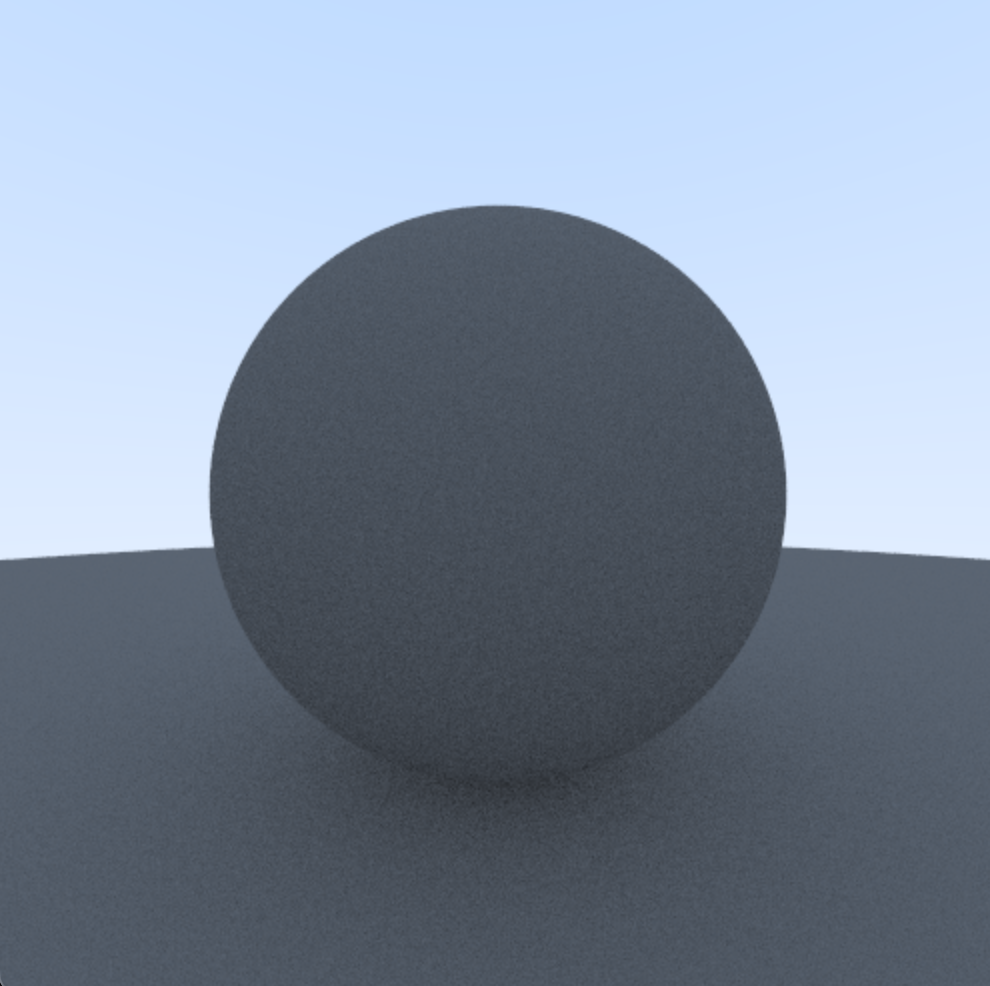
\includegraphics[width=\textwidth]{images/uniform_diffuse.png}
                  \caption{Rendered image using Uniform Diffuse Renderer}
                  \label{fig:completely_diffuse}
              \end{subfigure}
              \hfill
              \begin{subfigure}[b]{0.45\textwidth}
                  \centering
                  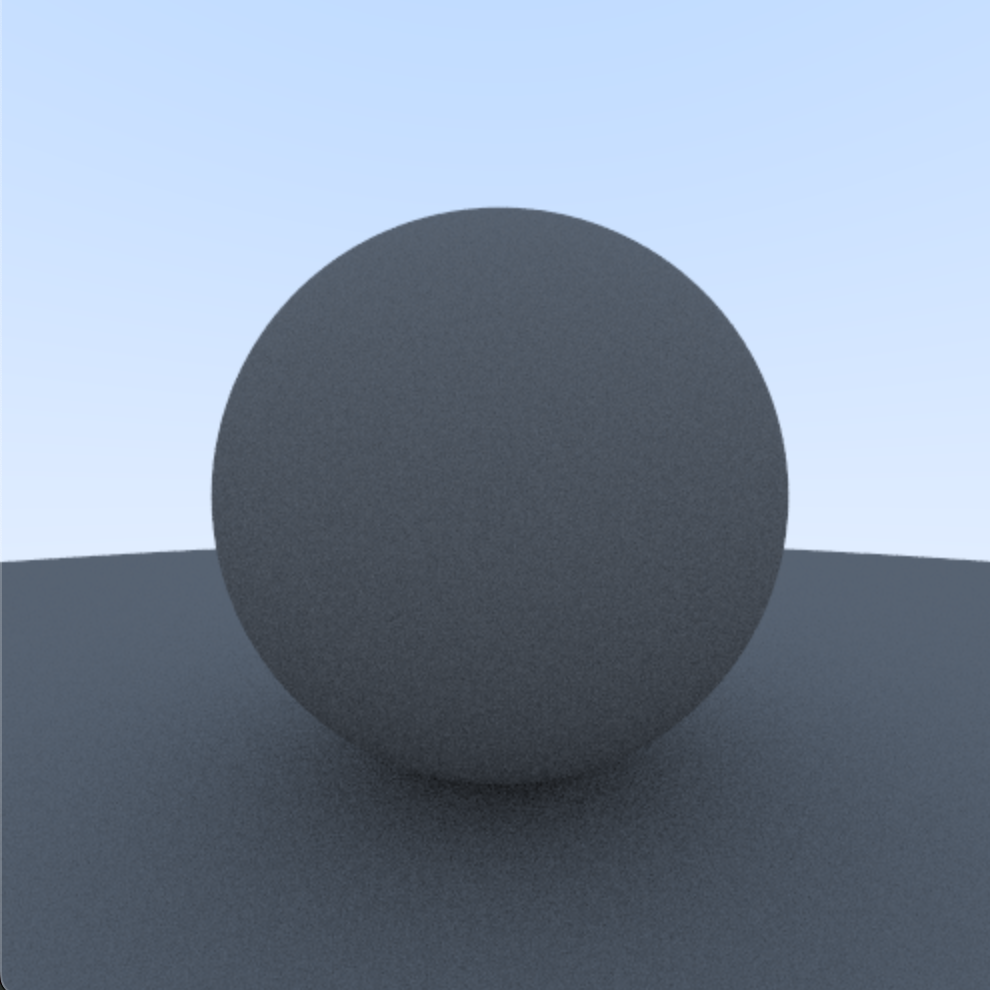
\includegraphics[width=\textwidth]{images/lambertian_diffuse.png}
                  \caption{Rendered image using Lambertian Diffuse Renderer}
                  \label{fig:lambertian_diffuse}
              \end{subfigure}
              \caption{Comparison of rendering techniques}
              \label{fig:rendering_comparison}
          \end{figure}
    \item \textbf{Metal:} Reflective surfaces modeled using Fresnel equations and other techniques.
\end{itemize}
\subsection{Linear Transformations}
\begin{itemize}
    \item \textbf{Translation, Rotation, and Scaling:} Basic transformations applied to objects and rays.
    \item \textbf{Matrix Representations:} Using matrices to represent and compute transformations.
\end{itemize}
\subsubsection{Technical Implementation}
\begin{itemize}
    \item \textbf{Transforming Objects and Rays:} Applying matrix operations to objects and rays in the scene.
    \item \textbf{Applying Transformations to the Scene:} Ensuring consistent transformations across all scene elements.
\end{itemize}

\section{Advanced Techniques in Ray Tracing}
\label{sec:advanced}
\subsection{Camera and Viewing}
\begin{itemize}
    \item \textbf{Camera Model and Rays:} Understanding the projection of rays from the camera into the scene.
    \item \textbf{Viewport and Field of View:} Configuring the camera parameters for different viewing perspectives.
\end{itemize}
\subsubsection{Technical Implementation}
\begin{itemize}
    \item \textbf{Ray Generation from Camera:} Algorithms to generate rays from the camera's position.
    \item \textbf{Perspective Projection:} Implementing perspective transformations for realistic viewing.
\end{itemize}
\subsection{Acceleration Structures}
\begin{itemize}
    \item \textbf{Bounding Volume Hierarchies (BVH):} An advanced structure for efficient intersection tests.
\end{itemize}
\subsubsection{Technical Implementation}
\begin{itemize}
    \item \textbf{Efficient Ray-Object Intersection Tests:} Using BVH for faster intersection calculations.
    \item \textbf{Building and Traversing BVH:} Methods for constructing and navigating BVH structures.
\end{itemize}
\subsection{Anti-Aliasing and Sampling}
\begin{itemize}
    \item \textbf{Aliasing Problems in Rendering:} Understanding the impact of aliasing and methods to mitigate it.
    \item \textbf{Supersampling and Adaptive Sampling:} Techniques to enhance image quality.
\end{itemize}
\subsubsection{Technical Implementation}
\begin{itemize}
    \item \textbf{Implementing Supersampling:} Methods for applying supersampling in rendering.
    \item \textbf{Random Sampling Techniques:} Utilizing stochastic methods to improve sampling efficiency.
\end{itemize}

\section{Mathematical Methods for Ray Tracing}
\label{sec:math-methods}
\subsection{Probability and Monte Carlo Methods}
\begin{itemize}
    \item \textbf{Basic Probability Concepts:} Foundational principles applicable to Monte Carlo methods.
    \item \textbf{Monte Carlo Integration:} Using random sampling to approximate integrals.
\end{itemize}
\subsubsection{Technical Implementation}
\begin{itemize}
    \item \textbf{Path Tracing:} Implementing Monte Carlo techniques in path tracing.
    \item \textbf{Importance Sampling and Russian Roulette:} Advanced Monte Carlo techniques to enhance efficiency.
\end{itemize}
\subsection{Integration for Lighting Models}
\begin{itemize}
    \item \textbf{Radiance and Light Transport Equations:} Mathematical models for light behavior.
    \item \textbf{Numerical Integration Techniques:} Applying numerical methods to solve lighting equations.
\end{itemize}
\subsubsection{Technical Implementation}
\begin{itemize}
    \item \textbf{Implementing Global Illumination:} Techniques for comprehensive lighting calculations.
    \item \textbf{Integrating Direct and Indirect Lighting:} Methods to account for all lighting contributions.
\end{itemize}

\section{Optimization Techniques}
\label{sec:optimization}
\subsection{Performance Optimization}
\begin{itemize}
    \item \textbf{Profiling and Bottleneck Identification:} Strategies for identifying and addressing performance issues.
    \item \textbf{Algorithmic Improvements:} Enhancing algorithms for better performance.
\end{itemize}
\subsubsection{Technical Implementation}
\begin{itemize}
    \item \textbf{Optimizing Intersection Tests:} Techniques to speed up intersection calculations.
    \item \textbf{Efficient Memory Management:} Methods to handle memory efficiently in rendering.
\end{itemize}
\subsection{Parallelization and Multithreading}
\begin{itemize}
    \item \textbf{Concepts of Parallel Processing:} Understanding parallel computing principles.
\end{itemize}
\subsubsection{Technical Implementation}
\begin{itemize}
    \item \textbf{Utilizing Multithreading for Ray Tracing:} Implementing multithreading to enhance rendering speed.
    \item \textbf{GPU Acceleration:} Leveraging GPU capabilities for faster rendering.
\end{itemize}

\section{Conclusion}
\label{sec:conclusion}
\subsection{Summary of Key Points}
Monte Carlo methods are effective for path tracing and realistic image synthesis. Importance sampling and stratified sampling significantly improve image quality and convergence speed. Variance reduction techniques further enhance the rendering efficiency by reducing noise.
\subsection{Future Work}
Future work could explore more advanced sampling strategies, real-time rendering optimizations, and additional variance reduction techniques.
\subsection{Final Thoughts}
The implementation of these techniques in a practical renderer highlights the importance of statistical methods in achieving high-quality, efficient rendering solutions.

\section{References}
\label{sec:references}
\bibliographystyle{plain}
\bibliography{references}

\appendix
\section{Detailed Mathematical Derivations}
\section{Code Snippets and Pseudocode}
\section{Additional Figures and Diagrams}

\end{document}